% !TEX TS-program = pdflatex
% !TEX encoding = UTF-8 Unicode
% !TEX root = main.tex
% !TEX spellcheck = en-US
% ****************************************************************************************
% File: thesis.tex
% Author: Patrick Haselwanter
% Date: 2023-10-28
% ****************************************************************************************
\documentclass[a4paper,11pt,oneside,final,titlepage,openany,onecolumn]{report}
% input preamble (include additional packages, set options, define macros)
\input{./tex/_preamble.tex}
\loadglsentries{./tex/_defns.tex}
\begin{document}
	\pagenumbering{alph}
	\include{./tex/titlepage.tex}
	\pagenumbering{Roman}
	\pdfbookmark[0]{\contentsname}{toc}
	\tableofcontents
	\newcounter{romanpagecount}
	\setcounter{romanpagecount}{\value{page}}
	\clearpage
	\pagenumbering{arabic}
	% add content of thesis here
    \chapter{Introduction}
\label{chap:Introduction}

This project focuses on the simulation of a steady-state 3D fluid flow and heat transfer problem within a flow heater, a configuration commonly found in process engineering applications. Accurately predicting both the flow field and temperature distribution is crucial to ensuring a homogeneous process environment, which directly impacts the overall quality of the process.

The geometry of the flow heater is shown in Figure \ref{fig:heater_geo}. For the purposes of this study, a 2D simplification (top-down view) was employed. This reduction in complexity allows for more efficient calculations and comparisons between different turbulence models, while maintaining a reasonable level of accuracy for the task at hand. The study primarily aimed to perform a Grid Convergence Study and evaluate various solver models, with results later applied to custom geometries for further simulations.

The flow heater in this case is examined under both laminar and turbulent flow conditions, leveraging different turbulence models to understand their effect on the heat transfer performance. The comparison of these models plays a key role in identifying the most appropriate solver configuration for real-world applications.

    \begin{figure}[h]   
    \centering
    \includegraphics[width=0.65\textwidth]{img/heater_geo_og.png}
    \caption{Given heater geometry}
    \label{fig:heater_geo}
\end{figure}

% EOF

	% !TEX TS-program = pdflatex
% !TEX encoding = UTF-8 Unicode
% !TEX root = ../main.tex
% !TEX spellcheck = en-US
% ****************************************************************************************
% File: func_descr_and_theor_aspects.tex
% Author: Patrick Haselwanter, Christoph Ehrhardt
% Date: 2023-10-28
% ****************************************************************************************
\chapter{Meshing of the Domain}
\label{chapter:meshing}

The meshing of the domain is a crucial step in the simulation process as it directly affects the accuracy of the results. 
The following settings were used:
\begin{itemize}
    \item item size of \qty{2}{\milli\meter}
    \item 5 inflation layers with growth rate 1,2
\end{itemize}

The mesh of the whole domain for the basic geometry is shwon in \autoref{fig:meshing_base_geometry_full_view} while \autoref{fig:meshing_base_geometry_detailed_view} shows a detailed view of the meshing at the walls and heater element.


\begin{figure}[htbp]   
    \centering
    \includegraphics[width=0.8\textwidth]{img/meshing_base_geometry_full_view}
    \caption{Full view of the base geometry meshing}
    \label{fig:meshing_base_geometry_full_view}
\end{figure}


\begin{figure}[htbp]
    \centering
    \includegraphics[width=0.8\textwidth]{img/meshing_base_geometry_detailed_view}
    \caption{Detailed view of the base geometry meshing}
    \label{fig:meshing_base_geometry_detailed_view}
\end{figure}

\section{Grid Convergence Study}
\label{sec:grid_convergence_study}

To ensure the mesh independency of the results, a grid convergence study according to \autocite{ExaminingSpatialGrid} was performed.
The mesh size was varied between \qty{4}{\milli\meter}, \qty{2}{\milli\meter} and \qty{1}{\milli\meter} whilst keeping the number of inflation layers constant. To evaluate the results, the area-weighted average static temperature across the flow \qty{25}{\milli\meter} before the outlet was used.
The results are shown in \autoref{tab:grid_convergence_study} and \autoref{fig:grid_convergence_graph}.

\begin{table}[htbp]
    \centering
    \caption{Grid convergence study}
    \label{tab:grid_convergence_study}
    \begin{tabular}{lcc}
        \toprule
        Mesh size & Temperature [\unit{\kelvin}] \\
        \midrule
        \qty{4}{\milli\meter} & 305.62 \\
        \qty{2}{\milli\meter} & 304.96 \\
        \qty{1}{\milli\meter} & 304.69 \\
        Richardson Extrapolation & 304.503 \\
        \bottomrule
    \end{tabular}
\end{table}

\begin{figure}
    \centering
    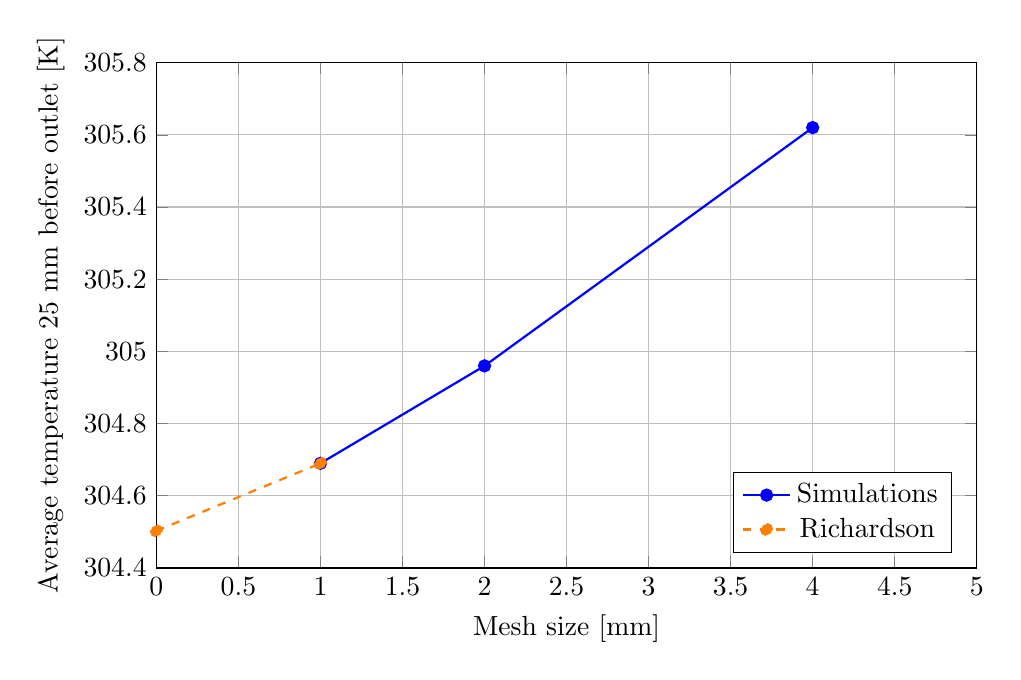
\begin{tikzpicture}
        \begin{axis}[
            width=12cm, height=8cm,
            xlabel={Mesh size [mm]},
            ylabel={Average temperature 25 mm before outlet [K]},
            legend pos=south east,
            grid=both,
            xmin=0, xmax=5,
            ymin=304.4, ymax=305.8
        ]
            % Simulations data
            \addplot[color=blue, mark=*, thick] coordinates {
                (1, 304.69)
                (2, 304.96)
                (4, 305.62)
            };
            \addlegendentry{Simulations}

            % Richardson extrapolation data
            \addplot[color=orange, dashed, mark=*, thick] coordinates {
                (0, 304.503)
                (1, 304.69)
            };
            \addlegendentry{Richardson}
            
        \end{axis}
    \end{tikzpicture}
    \caption{Grid convergence graph showing the variation of temperature with mesh size}
    \label{fig:grid_convergence_graph}
\end{figure}

The grid convergence study yields an asymptotic range of convergence of 0.99911, a \qty{0.19}{\percent} \gls{acr:gci} between \qty{4}{\milli\meter} and \qty{2}{\milli\meter} and a \qty{0.08}{\percent} \GLS{acr:gci} between \qty{2}{\milli\meter} and \qty{1}{\milli\meter} mesh sizing and thus shows that the results can be seen as mesh independent for a mesh size of \qty{2}{\milli\meter}.


% EOF
    % !TEX TS-program = pdflatex
% !TEX encoding = UTF-8 Unicode
% !TEX root = ../main.tex
% !TEX spellcheck = en-US
% ****************************************************************************************
% File: solver_comparison.tex
% Author:  Schmid 
% Date: 
% ****************************************************************************************
\chapter{Comparison of linear and turbulent model}
\label{chapter:solver_comp}

\paragraph{Estimating Reynolds Number}~

The Reynolds number is a critical dimensionless quantity in fluid dynamics that determines whether the flow is laminar or turbulent. It represents the ratio of inertial forces to viscous forces in the fluid and provides insight into the flow regime. In this study, the Reynolds number is essential to select an appropriate turbulence model, as different flow regimes (laminar or turbulent) significantly affect heat transfer and velocity profiles. Using an inaccurate Reynolds number can lead to incorrect model assumptions, which would undermine the accuracy of the simulation results. Thus, calculating and interpreting the Reynolds number is a fundamental step to ensure the validity of the chosen numerical approach.

The Reynolds number is calculated as:
\[
Re = \frac{\rho \cdot v \cdot L}{\eta}
\]
where:
\begin{align*}
\rho & = \text{Density of the fluid } [\text{kg/m}^3], \\
v & = \text{Velocity of the fluid } [\text{m/s}], \\
L & = \text{Characteristic length } [\text{m}], \\
\eta & = \text{Dynamic viscosity of the fluid } [\text{Pa·s}].
\end{align*}

If we would use the length of the heater (\SI{300}{\mm} as characteristic length we would have a turbulent mode with a Reynolds number around \SI{4000}{}. If we would narrow down the evaluation to the critical area arround the heating element, we would need to consider using the heater dimensions of \SI{10}{\mm} for the calculation, leading us to a Reynolds number of approximate \SI{137}{} which is way below the critical Re of \SI{2300}{}. This would indicate that we have a laminar flow.
Because we encounter wall effects and can not certainly determine a pure laminar flow behavior we will not the laminar model for the calculations. However we keep the laminar model for the basic comparison.


While solving a problem in the fluent domain it is necessary to choose a valid model. We could either use a linear model or a turbulent model.
This chapter deals with the comparison of a linear model, a turbulent k-omega (SST) model, a turbulent k-epsilon model and a turbulent k-kl-epsilon model.

\paragraph{Y+ consideration}~

To calculate Y+ we use the formula given in the support material for this course \cite{y_plus_calc}. This calculation assumes a \SI{2}{\mm} grid without inflation layer. Inflation layer would improve the Y+ value but because we use a questionable Reynolds Number this calculation is only used as coarse guidance and we use the Ansys simulation output later on to make a statement.

\textbf{Step 1: Reynolds Number (\( Re \))}
\[
Re = \frac{\rho \times U \times L}{\mu}
\]

\[
Re = \frac{1.225 \times 0.2 \times 0.1}{1.7894 \times 10^{-5}} = 1363.5
\]

\textbf{Step 2: Skin Friction Coefficient (\( C_f \))}
\[
C_f = 0.058 \times Re^{-0.2}
\]

\[
C_f = 0.058 \times 1363.5^{-0.2} = 0.00501
\]

\textbf{Step 3: Wall Shear Stress (\( \tau_w \))}
\[
\tau_w = \frac{1}{2} \times C_f \times \rho \times U^2
\]

\[
\tau_w = \frac{1}{2} \times 0.00501 \times 1.225 \times (0.2)^2 = 0.000122 \, \text{Pa}
\]

\textbf{Step 4: Friction Velocity (\( U_\tau \))}
\[
U_\tau = \sqrt{\frac{\tau_w}{\rho}}
\]

\[
U_\tau = \sqrt{\frac{0.000122}{1.225}} = 0.010
\]

\textbf{Step 5: Dimensionless Wall Distance (\( y^+ \))}
\[
y^+ = \frac{\rho \times U_\tau \times y}{\mu}
\]

\[
y^+ = \frac{1.225 \times 0.010 \times 0.002}{1.7894 \times 10^{-5}} = 1.37
\]



The laminar and k-omega model can be applied without further investigation of the y+ value. The y+ value quantifies the interaction between turbulence and the wall, therefore it is not applicable to a laminar model. The k-omega model uses enhanced wall treatment, therefore it is a 2-layer model which is not sensitive to the y+ value.
For the k-epsilon model we also applied enhanced wall treatment but due to the properties of the model we looked into the y+ value. The k-kl-omega model was applied with standard configuration and the y+ value was also investigated. Figure \ref{fig:k_epsilon_enhanced_y_plus} shows the critical region of the geometry with the plotted y+ values for k-epsilon model. The y+ values differes depending on the position and the critical length, the figure shows that the value is largely way below 1 and only is close to 1 at positions where you would expect the biggest influence of the wall to the (turbulent) flow.
The same applies to the y+ values for the k-kl-omega model as displayed in figure \ref{fig:k_kl_omega_y_plus}.

\begin{figure}[h]   
    \centering
    \includegraphics[width=0.7\textwidth]{img/y_plus_k_epsilon_enhanced_wt.png}
    \caption{y+ plot for k-epsilon with enhanced wall treatment}
    \label{fig:k_epsilon_enhanced_y_plus}
\end{figure}

\begin{figure}[h]   
    \centering
    \includegraphics[width=0.7\textwidth]{img/y_plus_k_kl_omega_detail_inf5.png}
    \caption{y+ plot for k-kl-omega}
    \label{fig:k_kl_omega_y_plus}
\end{figure}

\clearpage

For the comparison the basic geometry is used, the meshing is done according to the results of chapter \ref{chapter:meshing}.
To compare the results the velocity, pressure and temperature are plotted.

\paragraph{Temperature Plot}~

The static temperature distribution for all four models is presented in Figure \ref{fig:temp_plot}, with each window labeled for clarity. The laminar model produces the least symmetrical result, contrary to expectations given the geometry. This lack of symmetry appears to stem from eddies that disrupt the flow and cause uneven heat distribution.

The k-epsilon model with enhanced wall treatment shows a sharp temperature gradient immediately after the heaters, leading to a less uniform temperature profile across the outlet. While the outlet temperature matches the other models, the distribution (average across the outlet) is slightly lower.

Both the k-omega and k-kl-omega models deliver more uniform and physically consistent results. The k-kl-omega, while accurate, involves additional equations and computational effort, making it better suited for cases involving transitional flows. k-omega model provides a credible and computationally efficient solution.

\begin{figure}[htbp]   
    \centering
    \includegraphics[width=1\textwidth]{img/Temp_plot_comparison.png}
    \caption{Temperature plot for all 4 models}
    \label{fig:temp_plot}
\end{figure}

\paragraph{Velocity Plot}~

The velocity plot supports the observations from the temperature plot.
The velocity distribution in the laminar plot shows smooth transitions near the heating elements with minimal mixing. the k-omega model shows great mixing with well defined recirculation behind the heating element. k-l-omega is quit similar but does not offer the same amount of mixing.
The k-epsilon model shows a well-mixed flow after the heating elements, especially with the enhanced wall treatment the result seems trustworthy.


\begin{figure}[htbp]   
    \centering
    \includegraphics[width=1\textwidth]{img/Velocity_plot_comparison.png}
    \caption{Velocity plot for all 4 models}
    \label{fig:velocity_plot}
\end{figure}

\paragraph{Pressure Plot}~

The velocity and pressure plots are inherently linked through fluid dynamics principles, particularly Bernoulli's equation and the Navier-Stokes equations. In the presented simulations, regions of higher velocity correspond to areas of lower pressure due to the conservation of energy in the flow. This relationship is evident across all turbulence models, where pressure decreases as the flow accelerates past the heaters and recirculation zones are formed.

\begin{figure}[h]   
    \centering
    \includegraphics[width=1\textwidth]{img/Pressure_plot_comparison.png}
    \caption{Pressure plot for all 4 models}
    \label{fig:press_plot}
\end{figure}

\paragraph{Chosen Model}~

The k-omega model was chosen for its balance between accuracy and computational efficiency. It provides a credible and symmetrical result for the temperature, velocity, and pressure distributions, aligning well with theoretical expectations and the problem's physical constraints. Unlike the k-kl-omega model, which requires more computational resources due to additional equations, the k-omega model achieves comparable accuracy without the added complexity. This makes it a practical choice for simulations focusing on steady turbulent flow while maintaining reliable performance.


% EOF
	
	\include{./tex/methods.tex}
	%% !TEX TS-program = pdflatex
% !TEX encoding = UTF-8 Unicode
% !TEX root = ../main.tex
% !TEX spellcheck = en-US
% ****************************************************************************************
% File: measurements.tex
% Author: Patrick Haselwanter
% Date: 2023-10-28
% ****************************************************************************************
\chapter{Hardware Implementation and Results}
\label{chapter:measurements}
\section{Hardware Implentation}
\label{sec:HI}
The setup of the real hardware is shown in \cref{fig:measurement_test_setup}.
\begin{figure}[htbp]
	\centering
	\includegraphics[width=0.5\textwidth]{img/setup.jpg}
	\caption{Real hardware setup}
	\label{fig:measurement_test_setup}
\end{figure}
It is composed of a cylinder in which a table tennis ball can move up and down. A fan mounted under the cylinder serves as the actuator that moves the table tennis ball. The position of the ball is read by a sensor mounted above the cylinder. 
The fan is controlled via a separate power supply module. This converts the input voltage of 5V into a corresponding PWM signal depending on the control setpoint. The control setpoint is defined via a controller implemented in Simulink, Simulink communicates with an I/O module from National Instruments (NI) and this passes the analog output to the power supply module. 
There is a similar setup for reading out the sensor, here the analog signal is forwarded to Simulink via the I/O module from NI. 

To apply the controller described in chapter \ref{chap:contr_des} to a real system, the Simulink-file shown in chapter \ref{chap:sim} is used as a basic setup. Instead of the identified system of the real plant, some interfaces to the real plant have to be introduced. This is done with the \textit{Analog Input} block, which builds the interface to the distance sensor and an \textit{Analog Output} block, which builds the interface to the fan motor. For the hardware of the laboratory at MCI VI, the drivers for the I/O Module \textit{National Instruments PCI 6221} have to be installed on the PC. 

To be able to do the system identification described in chapter \ref{sec:sys_ident}, an offset and a gain had to be applied to the response of the system. In order to be able to use the same controller as for the identified system, this offset of $d=0.77$ and gain of $k=1.81$ has to be introduced now to the real system. In the Simulink model, this has been done with simple \textit{gain} and \textit{bias} blocks. 

The following figure shows the Simulink system with the introduced gain and offset-blocks. Additionally, this figure shows the analog in- and output blocks, needed as an interface to the real hardware. 
\begin{figure}[!h]
\centering
    \begin{subfigure}{\textwidth}
      \centering
      \includegraphics[width=1\linewidth]{img/real_layer1.png}
      \caption[Top level servo controlled system]{Top level servo controlled system with interface to the real hardware and introduced offsets ad gains}
      \label{fig:simlayer1}
    \end{subfigure}
    \begin{subfigure}{\textwidth}
      \centering
      \includegraphics[width=.8\linewidth]{img/real_layer2.png}
      \caption{Linear system with observer}
      \label{fig:simlayer2}
    \end{subfigure}   
    \caption[Simulink model used for the real hardware implementation]{Simulink model used for the real hardware implementation}
    \label{fig:Simulink_sim_model}
\end{figure}
%%%%%%%%%%%%%%%%%%%%%%%%%%%%%%%%%%%%%%%%%%%%%%%%%%%%%%%%%%%%%%%%%%%%%%%%%%%%%%%%%%%%
\section{Results}
\label{res}
To verify if the implemented control structure described in the previous chapter works properly on the real system, several input trajectory signals were defined, which the system was supposed to follow. 
\\In the following figure \ref{fig:step}, the system is supposed to follow step signals. 
\begin{figure}[!h]
\centering
    \begin{subfigure}{.5\textwidth}
      \centering
      \includesvg[width=1\linewidth]{img/01.svg}
      \caption{Step-reference 1}
      \label{fig:01}
    \end{subfigure}%
    \begin{subfigure}{.5\textwidth}
      \centering
      \includesvg[width=1\linewidth]{img/02.svg}
      \caption{Step-reference 2}
      \label{fig:02}
    \end{subfigure}
    \caption{Response to step trajectory references}
    \label{fig:step}
\end{figure}

As it can be seen, the hardware follows the trajectory with a certain overshoot . Additionally, differently from the simulation, the real hardware oscillates quite a bit around the desired step-setpoint.   case. In this figure, the voltage represents to the distance measured by the sensor. Through the sensor characteristic, this voltage can be converted to a distance value. The voltage to ball-height conversion can be seen in the following figure \ref{fig:volt_dist}. 
\begin{figure}[!h]
        \centering
        \includesvg[width=0.5\linewidth]{polyfit_sens_data.svg}
        \caption[Sensor voltage to ball-height characteristic]{Sensor voltage to ball-height characteristic}
        \label{fig:volt_dist}
\end{figure}

It can be seen that sensor does not follow a linear relationship between voltage and height. In addition to this nonlinear sensor characteristic, also the introduced offsets and gains have to be taken into account, when the voltage values are transformed into ball-height values. 
This voltage to height conversion can be applied equally also for the results described subsequently.  
In the following figure \ref{fig:04} the response to a reference trajectory consisting of several steps is shown. 
\begin{figure}[!h]
        \centering
        \includesvg[width=0.5\linewidth]{img/04.svg}
        \caption{Response to a trajectory containing several steps}
        \label{fig:04}
\end{figure}
\\In this figure it can be seen, that the system tries to follow the reference trajectory. However, since the time between the single steps is quite short, the hardware is not able to follow the reference trajectory perfectly. Especially in the first step, the system is not able to follow the reference and has a high overshoot. 
In the following figure \ref{fig:sine} the response to sinusoidal reference inputs is shown.

\begin{figure}[!h]
\centering
    \begin{subfigure}{.5\textwidth}
      \centering
      \includesvg[width=1\linewidth]{img/03.svg}
      \caption{Sine-reference - low freq and low amp}
      \label{fig:06}
    \end{subfigure}%
    \begin{subfigure}{.5\textwidth}
      \centering
      \includesvg[width=1\linewidth]{img/05.svg}
      \caption{Sine-reference 2 - middle freq and high amp}
      \label{fig:06}
    \end{subfigure}
    \begin{subfigure}{.5\textwidth}
      \centering
      \includesvg[width=1\linewidth]{img/06.svg}
      \caption{Sine-reference 3 - high freq and high amp}
      \label{fig:06}
    \end{subfigure}    
    \caption{Response to sinusoidal trajectory references}
    \label{fig:sine}
\end{figure}
As it can be seen, the hardware is able to follow the sinusoidal reference trajectory at low frequencies. However, if the trajectory-frequency is too high, the system response is too slow to follow the trajectory. Additionally, in all three frequency examples it can be seen, that the system has problems to follow the trajectory in the startup. In all cases, this results in a relatively high overshoot.  
    \include{./tex/discussion.tex}
    
	\pagenumbering{Roman}
	\setcounter{page}{\value{romanpagecount}}
	\stepcounter{page}

    %added from Jakob
    \printbibliography[heading=bibintoc] % This will add the bibliography to the table of contents
    
	%\bibliography{bib} % point BibTEX at the .bib files
	\addcontentsline{toc}{chapter}{\bibname}
	\listoffigures
	\addcontentsline{toc}{chapter}{\listfigurename}
	\listoftables
	\addcontentsline{toc}{chapter}{\listtablename}
	\clearpage
	\printglossary[type=acronym] % input files created by makeindex
	\printglossary[type=symbolslist,style=symbolsliststyle] % input files created by makeindex
	\appendix
	% !TEX TS-program = pdflatex
% !TEX encoding = UTF-8 Unicode
% !TEX root = ../main.tex
% !TEX spellcheck = en-US
% ****************************************************************************************
% File: appendix.tex
% Author: Patrick Haselwanter
% Date: 2023-10-28
% ****************************************************************************************

% EOF
\end{document}
% EOF